\section{Comparison between Nonlinear and Linearized System}

The Wang et. al paper suggests that the carrying capacity terms involving $K_A$ and $K_R$ are necessary to accurately produce incidence curves that fit epidemiological data. Given that our linearized system was neccesary for sensitivity analysis, but necessarily did not include these competition terms, we were interested in verifying if accurate behavior of the model was indeed nonrecoverable. 

\begin{figure}[h]
    \centering
    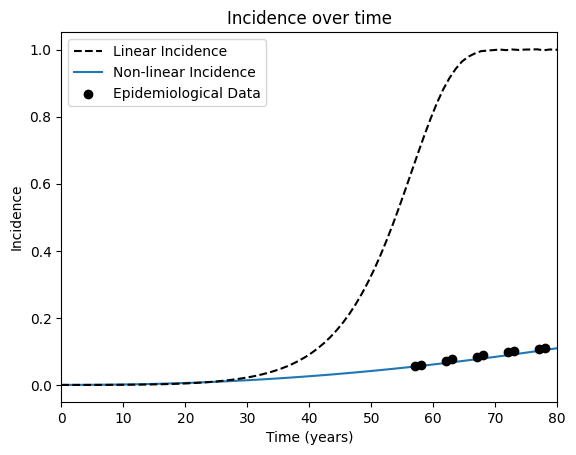
\includegraphics[width=0.65\linewidth]{figures/LinvsNonlin_Incidence.png}
    \caption{Comparison of incidence curves produced by the nonlinear and linearized systems.}
    \label{fig:linear sys empirical}
\end{figure}

\FloatBarrier 
From this figure, we see immediately that this competition term which couples mutant crypt populations is necessary to produce reliable incidence curves. Without this term, mutant crypt populations grow exponentially without limit, leading to a steep increase in the probability of having a type six crypt form. In the linear case, this probability reaches 1 within a human lifetime. This, thankfully, vastly exceeds observed incidence rates which do not climb above 0.2 within a normal human lifetime.

While we confirmed that the linearized system does not produce a relevant incidence curve, we were interested to see if the results of our sensitivity analysis could be applied to both cases.